%%%%%%%%%%%%%%%%%%%%%%%%%%%%%%%%%%%%%%%%%
% Modified from example by Ted Pavlic
% by D. Runfola. 
%%%%%%%%%%%%%%%%%%%%%%%%%%%%%%%%%%%%%%%%%

%----------------------------------------------------------------------------------------
%	PACKAGES AND OTHER DOCUMENT CONFIGURATIONS
%----------------------------------------------------------------------------------------

\documentclass{article}
\usepackage{graphicx}
\usepackage{fancyhdr} % Required for custom headers
\usepackage{lastpage} % Required to determine the last page for the footer
\usepackage{extramarks} % Required for headers and footers
\usepackage{courier} % Required for the courier font

% Margins
\topmargin=-0.45in
\evensidemargin=0in
\oddsidemargin=0in
\textwidth=6.5in
\textheight=9.0in
\headsep=0.25in

\linespread{1.1} % Line spacing



 
\pagestyle{fancy}
\fancyhf{}
\rhead{Page \thepage}
\lhead{Lab 1 - William and Mary}

\begin{document}

\begin{center}
{\Huge Breaking Intuition - COLL 100}\\
\vspace{5mm}
{\huge Lab 5 - Thinking Spatially}\\ % Assignment title
\vspace{5mm}
\textit{Due: Friday, November 13th (before Lecture Begins)}\\
\vspace{25mm}
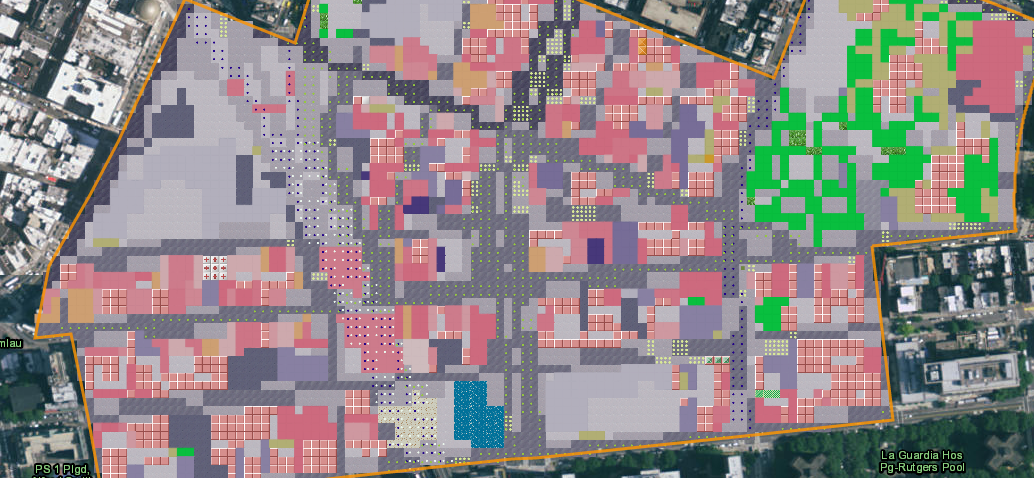
\includegraphics[scale=0.65]{Planning.png}
\end{center}



\newpage


\textbf{Objectives}

\textit{In this lab, you will:}
\begin{itemize}
\item Use GIS to design a city. 
\item Try to spatially optimize different characteristics of a city.
\item Consider the characteristics you personally believe are optimal in a city. 
\item Critically consider differences between perceived preferences and preferences revealed through the use of data.
\end{itemize}

\vspace{3mm}
\textbf{Materials}

\textit{To finish this lab, you will need:}
\begin{itemize}
\item A free account at https://visionmaker.us/nyc/
\item ....
\end{itemize}

\vspace{3mm}
\textbf{Grading}\\
This lab will be graded based on X sub-steps.  In the \textbf{first} step, you will specify your own intuitions regarding preferences in an urban area.  In the \textbf{second} step, you will attempt to design an urban area around those preferences.  ......  In each step, you will be graded according to the COLL Curriculum Rubric, found along with your syllabus.

\vspace{3mm}
\textbf{Step 1: What do you like in a city? (10 points)}\\
You have 100 points to distribute across the following categories - give more points to the things you value most in a city, and fewer points to those you value less:\\
\underline{\hspace{0.35cm}} Entertainment or other Venues.\\
\underline{\hspace{0.35cm}} Restaraunts.\\
\underline{\hspace{0.35cm}} Sports. \\
\underline{\hspace{0.35cm}} Walkability / walking to campus or work. \\
\underline{\hspace{0.35cm}} Greenspace.\\
\underline{\hspace{0.35cm}} Bike Lanes.\\
\underline{\hspace{0.35cm}} Clean Air or Low Carbon Emissions.\\
\underline{\hspace{0.35cm}} Ample Parking.\\
\underline{\hspace{0.35cm}} Lower-density housing.\\
\underline{\hspace{0.35cm}} High-density housing.\\

\newpage
\textbf{Step 2: Build new cities. (60 points)}\\
Using the rankings you have above, attempt to optimize an urban environment that contains all of the factors you desire.  You must build two cities, each under a different set of constraints, and consider how close (or far) from optimal you were able to get.  For the first city, load ... on visonmaker and....\\
For the second city....\\
NOTE: constraints would include things like population.  General idea would be to set aside specific areas of NYC to simulate a "small" or "medium" city, and force students to try and design for things that are particularly difficult - i.e., they must have a certain (large) population, or minimize floodwater concerns.  It would be good to accompany the below itemized steps with screenshots where possible.\\
To build your city, follow these steps:
\begin{itemize}
\item ...
\item ...
\item ...
\item ...
\item ...
\item ...
\item ...
\end{itemize}
\vspace{3mm}

\textbf{Step 3: Are your preferences possible? (20 points)}\\
Using your two cities as examples, discuss the feasability (or lack thereof) of your personal preferences.  Is it possible to achieve the perfect urban area for you?  If so, what conditions must be met?  If not, why not?  Discuss, and write a two page response using your data and figures.  




%----------------------------------------------------------------------------------------

\end{document}